\section{Introduction}

% Motivation
The University of Melbourne's cold-atom electron source aims to be able to create high-brightness, high-coherence electron bunches for use in coherent electron diffractive imaging. The imaging of nanoscale objects such as biological molecules\cite{dwyer_femtosecond_2006, williamson_clocking_1997} and defects in solid-state devices\cite{siwick_atomic-level_2003} by ultrafast, single-shot electron diffractive imaging would provide important information about structure and dynamic processes of these nanoscale objects.

In order to determine the structure of biological molecules atomic, sub-nanometre imaging resolution is required. A number of techniques are available for determining these structures \cite{nettleship_methods_2008, svergun_small-angle_2003, opella_structure_2004} and the most successful to date has been x-ray crystallography \cite{kendrew_three-dimensional_1958, uson_advances_1999}. Unfortunately the process of crystallising biological proteins such as membrane proteins is difficult and to date relatively few have been successfully crystallised \cite{geerlof_impact_2006}.

Membrane proteins are the proteins that are associated with or attached to the membrane of a cell. They are involved in detecting and conveying external signals into cells which allows the cell to interact with and respond to their environment\cite{almen_mapping_2009}. Membrane proteins are important in determining immune responses, interactions with pharmaceuticals, cell adhesion to form tissues and in controlling important metabolic processes such as salt balance, energy production and photosynthesis\cite{chiras_human_2011}. Determining the structure of these molecules is a key step in understanding their chemical and biological function. The importance of knowing the atomic structure of biomolecules is exemplified by the enormous progress made in various fields of biology once the double-helical structure of DNA was determined from x-ray images in 1953\cite{watson_molecular_1953}. Once a protein's structure and function are known then it becomes possible to design drugs\cite{pinto_influenza_1992} where needed and to more fully understand how the protein behaves in its biological system.

New imaging techniques and light sources such as x-ray free electron lasers and  ultrafast single-shot diffraction have been driven by the goal of overcoming the limitations of x-ray crystallography. Ultrafast single-shot diffraction imaging also has the potential to determine the dynamic structure of biological molecules.

\subsection{Ultrafast, single-shot, coherent diffractive imaging with electrons}
X-ray diffraction from crystals was first observed a century ago\cite{bragg_x-rays_1912} and resulted in a Nobel prize being awarded to William Bragg and his son. Since then \gls{cdi} has been performed on a myriad of different samples with coherent beams of x-rays and electrons.

Electron interactions with molecules are significantly strong than those of x-rays. For similar energies the electron interaction with a sample is $10^5-10^6$ higher than that of x-rays\cite{sciaini_femtosecond_2011}.

\subsubsection{Single-shot diffractive imaging}
Single-shot diffractive imaging with an x-ray source of sufficient brightness should be able to produce a diffraction pattern from scattered x-rays from a single molecule before the molecule is destroyed by the Coulomb explosion which follows photoionisation within the molecule\cite{henderson_potential_1995, neutze_potential_2000}. Single-shot imaging aims to avoid the need for crystallisation with x-ray imaging since with a sufficiently bright source imaging of any molecule would be possible.

With femtosecond timescale single-shot imaging it is possible to observe such things as molecular vibration and dynamic chemical processes\cite{zewail_4d_2006}. With the sophisticated imaging techniques currently in development it will become possible to create ``molecular movies''\cite{dwyer_femtosecond_2006} of these processes.

\subsection{Melbourne cold-atom electron source}
The University of Melbourne's cold-atom electron source project aims to produce an electron source for coherent diffractive imaging. If bright, coherent, femtosecond long bunches of electrons can be produced then \gls{cdi} can be performed on a range of structures.

In order to produce the electrons Rubidium atoms from an oven are first slowed using a Zeeman slower which consists of a near-resonant laser beam and a tapered magnetic coil. The Zeeman slower slows the atoms leaving the oven from speeds of order 300m/s to speeds of order 10m/s which correspond to a few Kelvin.

The slowed atoms are then cooled and trapped in a magneto-optic trap which consists of three sets of counter-propagating, circularly polarised, near-resonant laser beams combined with a magnetic field generated by two magnetic coils in an anti-Helmholtz arrangement. This serves to cool and trap the atoms to a temperature of order 100 $\mathrm{\mu}$K forming an ultra-cold atom-cloud.

With the atom cloud produced the electron beam production can begin. The cloud is first illuminated by a resonant 780 nm excitation laser to excite the valance electrons to a high energy level followed by a 480 nm ionisation laser pulse which provides just enough energy to ionise the electrons. Since the electrons are have little or no excess energy once they have been ionised they are considered to be `cold'.

These cold electrons are then accelerated out of the cloud by a uniform electric field, guided to the neighbouring sample chamber and focused onto the target sample. After passing through the sample the resulting diffraction pattern is incident upon the detector.

The diffraction pattern recorded by the detector can be used to determine the structure of the sample.

\begin{figure}[h]
	\centering
	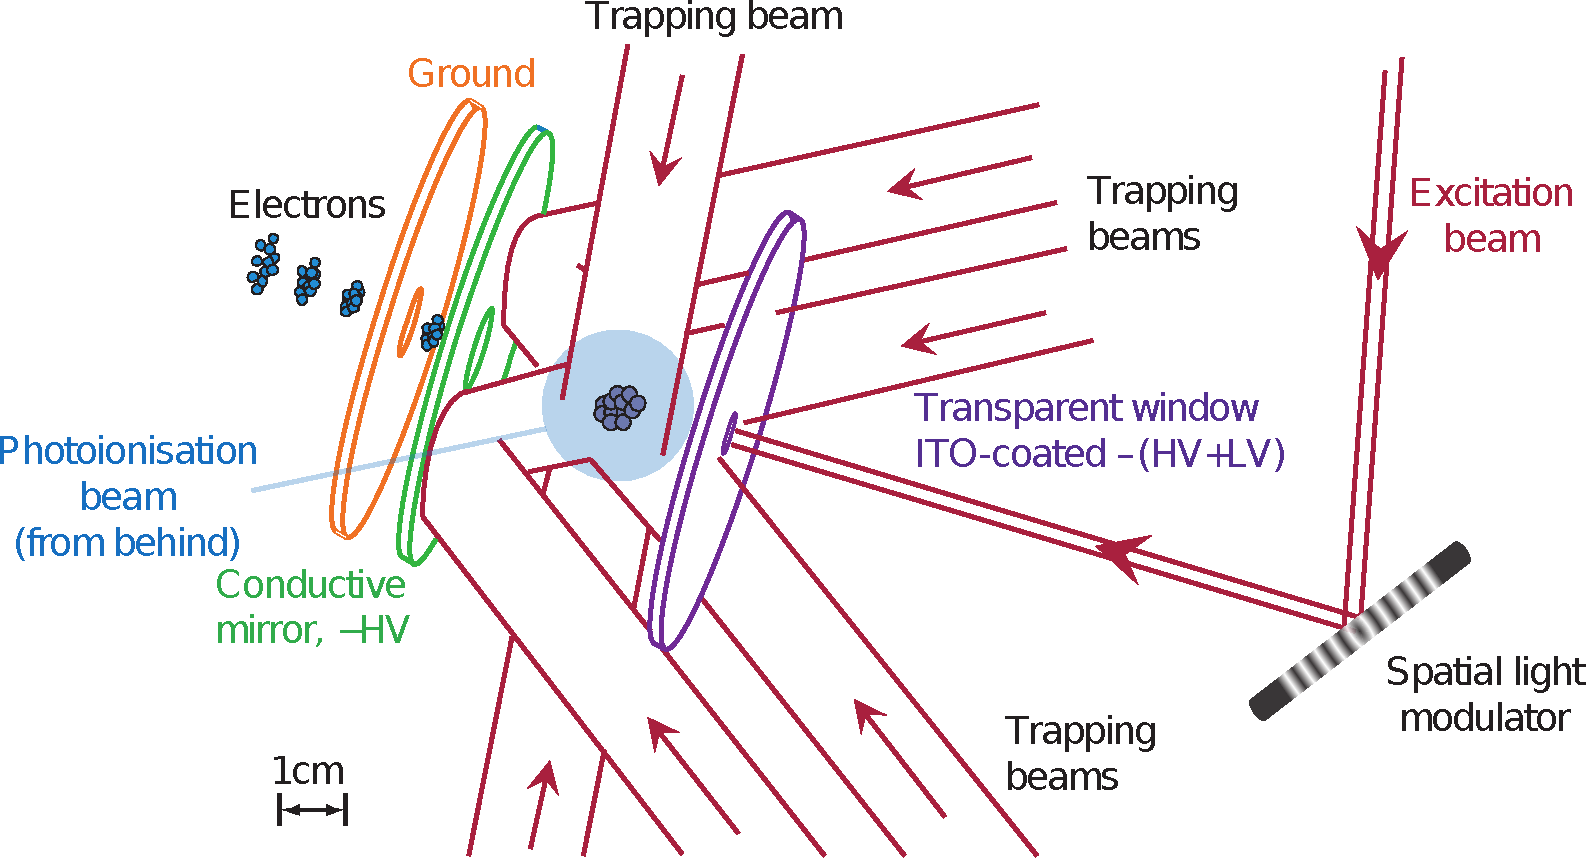
\includegraphics[scale=0.50]{{figs/MOT.pdf}}
	\caption[Title]{A quasi mirror MOT is used to trap Rb atoms. The atoms are then ionised and the resulting electrons are accelerated using two parallel plates.}
	\label{figs/MOT.pdf}
\end{figure}

